
\chapter{Theoritical Overview}
\label{sec:org2ae82f1}
\section{Units in particle physics}
\label{sec:org2338bc0}
Particle physics, study the properites of subatomic particles and their interactions. To describe such microscopic phenomena and quantities, an appropriate system of units must be adopted, for if the SI system of units was to be used, one would have to deal with large exponents. More over, it is more practical to utilize a system that is based on the typical length and time scales found in particle physics\cite{thomson_2013}.

The foundamental constants of the special theory of relativity, as well as quantum mechanics are \(\hbar\), c, and  GeV and they can be used as a basis to form a system of units, the Natural Units. Natural units can be further simplified by chosing:
\[ c = \hbar = 1\]
The table below sumarizes the relationship between natural units and S.I

\begin{table}[h!]
\centering
\begin{tabular}{ |p{3cm}|p{4cm}|p{3cm}|  }
 \hline
 \multicolumn{3}{|c|}{Relationship between natural units and S.I} \\
 \hline
 \hline
Quanity & Natural units($ \hbar = c = 1 $) & S.I \\
 \hline
Energy & GeV & $Kg m^{2}s^{-2}$ \\
Momentum & GeV& $ Kg m^{2}s^{-2}$ \\
Mass & GeV & Kg\\
Time & $GeV^{-1}$ & s\\
Length & $GeV^{-1}$ & m\\
 \hline
\end{tabular}
\caption{Some basic quantites in S.I and in Natural units .}
\label{table:natural_units}
\end{table}

\section{Special Relativity}
\label{sec:orgd8ae263}

\subsection{Four-Vectors - Lorentz transformations}
\label{sec:orgec107fd}

Let S and S' be two inertial reference systems, with S' moving at (a relativistic) 2velocity \(u\) relative to S. The coordinates are chosen such that the motion is along the x-axis in both reference systems. The clocks of both S and S' are synchronized so that when \(x = x' = 0\), \(t = t' = 0\).
For an event with coordinates (x, y, z, t) in S, the coordinates in S' are given by the Lorentz transformations:

\begin{equation}
\begin{matrix}
(x')^{0} = \gamma(x^{0} - \beta x^{1}) \\
(x')^{1} = \gamma(x^{1} - \beta x^{0}) \\
(x')^{2} = x^{2} \\
(x')^{3} = x^{3}
\end{matrix}
\end{equation}
where \(\beta \equiv \frac{u}{c}\text{,   } x^{0}\equiv ct\text{,    } x^{1}\equiv x\text{,   } x^{2}\equiv y\text{,   } x^{3}\equiv z\)

The elements \(x^{i}\text{, i = 0, 1, 2, 3}\) define the position four vector. Mathematicaly four vectors are 4 dimentional, rank 1 tensors that transform according to lorentz transformations

With the introduction of four vectors, using Einstein's summation convention, lorentz transformations can be written as:
\begin{equation}
(x')^{i} = \Lambda^{i}_{j}x^{j}
\end{equation}
Where \(\Lambda\), is the Lorentz transformation matrix, a rank 2 tensor:

\begin{equation}
\Lambda = \begin{pmatrix}
 \gamma & -\gamma \beta &  0 & 0 \\
  -\gamma \beta & \gamma &   0 & 0 \\
  0 & 0& 1 &0\\
  0 & 0& 0 &1\\
  \end{pmatrix}
  \end{equation}

The following quantity does not change under lorentz transformation:
\begin{equation}
I^{2} = -(x^{0})^{2} + (x^{1})^{2} + (x^{2})^{2} +(x^{3})^{2} = -(x'^{0})^{2} + (x'^{1})^{2} + (x'^{2})^{2} +(x'^{3})^{2}
\end{equation}
or written in a more compact form:
\begin{equation}
I = g_{\mu \nu}x^{\mu}x^{\nu} = x^{\mu}x_{\mu}
\end{equation} 
where \(g_{\mu\nu}\) is the Minkowski (metric) tensor:

\begin{equation}
g_{\mu \nu} = \begin{pmatrix}
-1 & 0 & 0 & 0\\
0 & 1 & 0 & 0\\
1 & 0 & 1 & 0\\
1 & 0 & 0 & 1\\
\end{pmatrix}
\end{equation}
Such a quantity as I is called \textbf{invariant}

The introduction of four vectors and the metric tensor, yield the Minkowski Space Time where points need 4 coordinates to be fully described(1, time like and 3 space like ) and the distance between them is beeing defined by the Minkowski tensor. The necessity of four vectors, in order to describe non scalar quantities(such as velocity and momentum) in minkowski space time, is therefore evident.

\subsection{Energy and Momentum}
\label{sec:org15fe0da}

According to the principle of relativity, the laws of physics must be the same in all inertial reference systems. Hence, if momentum is conserved  in one inertial frame of reference, it must also be conserved in all others. It is evident that the momentum of a moving particle must be defined in an appropriate manner, to satisfy the principle of relativity \cite{gParticles}. The four momentum is therefore defined as:
\begin{equation}
p^{\mu} = m\eta^{\mu}
\end{equation}
Where \(\eta^{\mu} = \frac{dx^{\mu}}{dt'}\), the four velocity of the particle.

The timelike component of four momentum, expresssed in natural units  is \(p^{0} = \gamma m\). The 3 space like components, constitue the vector momentum, \(\vec{p} = \gamma m\vec{\beta}\).
The relativistic energy is defined as:
\begin{equation}
E = \gamma m = p^{0}
\end{equation}
Thus, the components of four momentum are:
\begin{equation}
p^{\mu} = (E, \vec{p})
\end{equation}

At this point we are able to calculate the invariant "interval" \(p^{\mu}p_{\mu}\) :
\begin{equation}
p^{\mu}p_{\mu} = E^{2} - |\vec{p}|^{2} = m^{2}
\end{equation}
What is invariant in the case of momentum four vector, is the particle's mass. This quantity is called \textbf{invariant mass} of a particle as all observers, in different frames of references, agree upon its value. It is the invariant mass of particles that we can(or we try to) measure, in CERN as well. 

\section{The standard model}
\label{sec:org8632faf}

The Standard Model (SM)of particle physics is a theoretical framework that describes the fundamental particles and their interactions through the strong, electromagnetic, and weak forces. Each force is described by a corresponding quantum field theory(QFT). Namely, electromagnetic and weak interactions are described by the electroweak theory and the strong interactions by quantum chromodynamics(QCD). The interactions between particles in each QFT, are described in terms of the exchange of a spin-1 gauge boson. The photon, is the gauge boson of QED, while the gluon, which like the photon has no mass, is the force-carrying particle in the strong interaction. The charged \(W^{+} \text{and }W^{-}\) bosons mediate the weak charged current interaction, which is responsible for \(\beta\) decay and fusion, while the weak neutral current interaction, is mediated by the electrically neutral Z boson. These interactions are also governed by the principles of symmetry and conservation, which dictate that certain properties, such as charge and energy, are conserved during particle interactions

The fundamental particles that comprise all matter according to SM are the already mentioned gauge bosons, quarks, and leptons. The quarks and leptons are organized into three generations, with each generation containing two types of leptons and two types of quarks. The leptons are either negatively charged, with a charge of -1, or electrically neutral. The quarks, on the other hand, have fractional charges of either -1/3 or +2/3, and are characterized by their color, which can be blue, green, or red. Additionally, for each elementary fermion, there is a corresponding antifermion with the same mass and spin but with an opposite electric charge.
\begin{figure}[ht]
\centering
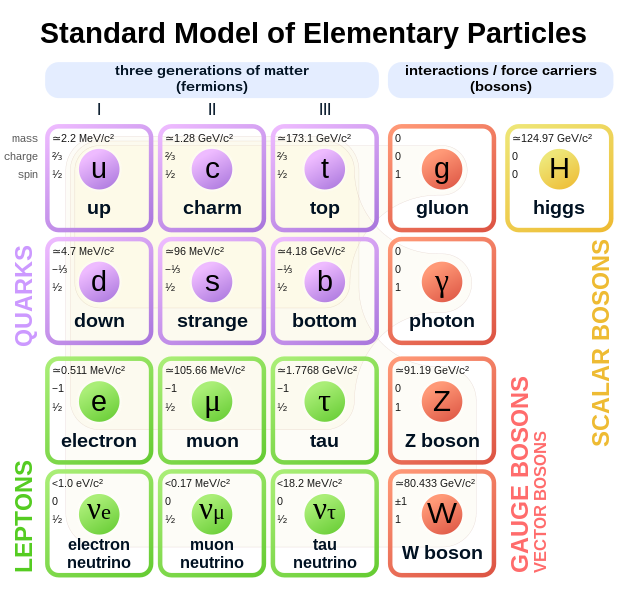
\includegraphics[width=0.35 \textwidth, ext=.png type=png]{/home/kpapad/UG_thesis/Thesis/Dissertation/src/figures/627px-Standard_Model_of_Elementary_Particles.svg.png}
\caption{Summary of the elementary particles. All matter around us is made up by 12 fermions!}
\label{fig:particles}
\end{figure}


Completing the picture of fundamental particles is the scalar boson, the Higgs boson, responsible for giving mass to the other particles. A brief summary of the fundamental particles is presented in Figure \ref{fig:particles}.

The SM has undergone extensive testing through high-energy experiments at CERN, with its predictions confirmed with a high degree of precision. However, the model has limitations, such as its inability to account for dark matter or the observed imbalance between matter and antimatter in the universe.

Despite its limitations, the Standard Model remains a cornerstone of modern physics, and its continued study and refinement is essential to advancing our understanding of the universe at its most fundamental level.
